\chapter{The D-Wave Quantum Computer}


% TODO: intro del capítulo


\section{Quantum Annealing}


Simulated annealing (SA) is an general optimization technique that was first introduced in 1983 by Kirkpatrick \emph{et al.} \cite{Kirkpatrick1983}. The main idea is to mimic how thermal fluctuations work to let the system escape from local minimums in the cost function. The \emph{temperature} of the system dictates the probability with which the is allowed to jump to worse solutions (higher values of the cost function). The \emph{annealing schedule} is the decrease rate of the temperature, controlled by the programmer. Under the appropiate one, the system would be able to scape from local minimums to reach the global one. If the temperature decreases too quickly, the system converges prematurely to a local minimum. If it decreases too slowly, the technique transforms into a random walker, reaching the global minimum at some point but being worthless time-wise.

Inspiration in thermal fluctuations are used in SA so the system may escape from local minima. Similarly, \emph{quantum tunneling} is used in Quantum Annealing (QA) in order to escape from local minimums. This new technique was introduced in its present form by two similar proposals \cite{Finnila1994} \cite{Kadowaki1998}.

Quantum tunneling is a quantum mechanical phenomenon where a wavefunction (i.e. a quantum state) may propagate through a potetial barrier \cite{Nimtz2008}. The probability of this event occuring depends on the height and width of the barrier (see figure \ref{fig 2.1})

\begin{figure}[h]
	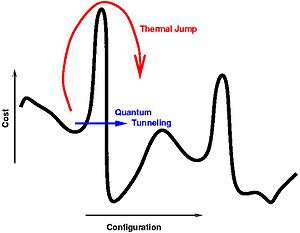
\includegraphics[scale=.8]{QuantumTunneling.jpg}
	\centering
	\caption{Thermal jumps vs quantum tunneling.}
	\label{fig 2.1}
\end{figure}

The main advantage of quantum tunneling compared to classical thermal fluctuations is that the probability of the system shifting depends to only on the height of the potential barrier but also on its width. Thus, application of QA may pottentially outperform SA in problems where the energy (cost) landscape consists on very high and thin barries surronding local minimums. 

Particularly, as studied in \cite{Ray1989}, let $\Delta$ be the height of a barrier and $\omega$ its width. The probability of a thermal transition ocurring is dictated by $exp\{-\frac{\Delta}{k_B T}\}$ where $T$ y the temperatue of the system and $k_B$ is the Boltzmann constant. On the other hand, the probability of a quantum tunneling transition ocurring through the same barrier (asumming isolation) is $exp\{-\frac{\sqrt \Delta \omega}{\Gamma}\}$, where $\Gamma$ is the tunneling field. Thus, the probability is much higher for the quantum tunneling effect on a high and thin barriers.

We may also observe looking at the previous expressions how the tunneling field and the temperature play a similar roles in the different methods. Thus, the annealing schedule of the QA system is controlled using the tunneling field just like the temperature is used in SA.

There are many examples in the literature of QA simulations using classical computers, both theoretical \cite{Morita2008} and numerical -most of them using Quantum Monte Carlo (QMC) methods \cite{Isakov2016} \cite{Farhi2000}-. This evidence suggests outperformance of SA by simulated QA under certain conditions. It is resonable to wonder what happens if instead of simulating QA we could somehow encode our problems in a real physical system that tends to its lower energy state (ground state), thus using quantum tunneling naturally. This is precisely what the D-Wave system does.

Let us farther deepen into the technicalities of quantum annealing in order to understand how it is implemented in the D-Wave system.


\section{Adiabatic Evolution}


The alternative form of the third postulate of quantum mechanics (section \ref{postulate-3'}) stated that the evolution of a quantum system is described by the Schrodinger equation:

$$ i \hbar \frac{d|\varphi\ra}{dt} = H|\varphi\ra $$

By better understanding the Hamiltonian $H$ we may controll this evolution. Suppose that at the evolution of a given quantum system is described by a Hamiltonian $\hat H(t)$. Suppose that at some initial time $t_0$ our quantum system is in an eigenstate $|\varphi(t_0)\ra$ of $\hat H(t_0)$. Since the evolution is continuous, at some other time $t_1 > t_0$ we could expect our system to be in the corresponding eigenstate $|\varphi(t_1)\ra$ of $\hat H(t_1)$. This fact critically depends on the time $\tau = t_1 - t_0$ during which the modification takes places, as stated by the adiabatic theorem, first proposed by Max Born and Vladimir Fock (1928) \cite{Born1928}.

\begin{theorem}[Adiabatic Theorem]
\label{adiabatic-theorem}
	A physical system remains in its instantaneous eigenstate if a given perturbation is acting on it slowly enough and if there is a gap between the eigenvalue and the rest of the Hamiltonian's spectrum.
\end{theorem}

Thus, we may define diabatic and adiabatic processes depending on how they adapt to the system changes \cite{Kato1950}.

\begin{definition}
	A \emph{diabatic process} is a process where rapidly changing conditions prevent the system from adapting its configuration during the process. Typically there is no eigenstate of the final Hamiltonian with the same functional form as the initial state. The system ends in a linear combination of the states.
\end{definition}

\begin{definition}
	An \emph{adiabatic process} is a process where gradually changing conditions allow the system to adapt its configuration. If the system starts in an eigenstate of the initial Hamiltonian, it will end in the corresponding eigenstate of the final Hamiltonian.
\end{definition}

The 'gap condition' that appears in theorem \ref{adiabatic-theorem} refers to an additional requirement: the spectrum of $\hat H(t)$ is \emph{nondegenerate}, meaning there are no two equal eigenvalues at fixed time $t$. This condition is also called the \emph{no-crossing} condition, and allow us to sort the eigenstates using the eigenvalues without any ambiguity.

As a classical annalogy, consider a simple pendulum. If the pendulum's support point is moved, the oscillation of the pendulum may change. In fact, violent changes on the support point will dramatically affect the pendulum's movement, changing it completely. However, if the support point is moved slowly enough, the pendulum will remain unchange. These are examples of diabatic and adiabatic processes respectively.


\subsection{Avoided crossing}


Let us consider a important physical example known as the \emph{avoided crossing}. Consider a two-state quantum system, i.e. a qubit. Suppose its Hamiltonian to be:

$$
	H = 
	\begin{pmatrix}
		E_1 & 0 \\
		0 & E_2 
	\end{pmatrix}
$$

Whose eigenvalues are $E_1$ and $E_2$, and eigenvectors,

$$
	|0\ra = 
	\begin{pmatrix}
	1 \\
	0 
	\end{pmatrix}, \quad
	|1\ra = 
	\begin{pmatrix}
	0 \\
	1 
	\end{pmatrix}
$$

which will be used as our base. Thus, a state vector describing the system may be written as a superposition of both states:

$$ |\varphi\ra = \alpha(t)|0\ra + \beta(t)|1\ra $$

Supposing adiabatic evolution, if the system is prepared in either one of the eigenstates it will remain as such as long as the gap condition is suffied: $E_1 \neq E_2$. However, if $E_1 = E_2$, any superposition of states will be an eigenstate, thus remaining unchanged. Hence, independently of $E_1$ and $E_2$, any system prepared in an eigenstate will remain as such, supposed adiabatic evolution.

Let us consider a $P$ perturbation into our original system. For simplicity we only consider perturbations with degenerated diagonal. Our new Hamiltonian will be the following:

$$
	H' = H + P =
	\begin{pmatrix}
	E_1 & 0 \\
	0 & E_2 
	\end{pmatrix} +
	\begin{pmatrix}
	0 & \omega \\
	\overline \omega & 0 
	\end{pmatrix} = 
	\begin{pmatrix}
	E_1 & \omega \\
	\overline \omega & E_2 
	\end{pmatrix}
$$

where $\omega \in \C$. Note that by setting $\omega$, the other value in the antidiagonal is fixed since $H'$ must be Hermitian. By using the characteristic equation we may compute the eigenvalues of $H'$:

$$ E_+ = \frac{1}{2}(E_1 + E_2) + \frac{1}{2}\sqrt{(E_1 - E_2)^2 + 4|\omega|^2} $$
$$ E_- = \frac{1}{2}(E_1 + E_2) - \frac{1}{2}\sqrt{(E_1 - E_2)^2 + 4|\omega|^2} $$


A continuación quiero añadir una imagen, seguramente como la de \href{https://en.wikipedia.org/wiki/Avoided_crossing}{wikipedia} (figura \ref{temp}):

\begin{figure}[H]
	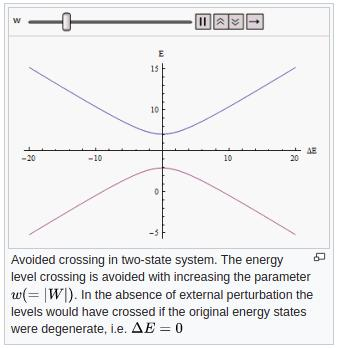
\includegraphics[scale=1]{wiki.jpg}
	\centering
	\caption{Figura de wikipedia}.
	\label{temp}
\end{figure}

He hecho una versión propia en Geogebra, tomando $E_1 = -E_2$ (luego $E_1 + E_2 = 0$ y $E_1 - E_2 = 2E$, he llamado $x \equiv 2E$). En la simulación, podemos ajustar el valor de $\omega$, que he llamado $a$ utilizando el slider, reproduciendo el efecto del gif de \href{https://en.wikipedia.org/wiki/Avoided_crossing}{wikipedia} (figura \ref{temp}):

\href{https://www.geogebra.org/graphing/svkrnu3s}{https://www.geogebra.org/graphing/svkrnu3s}

Sin embargo, me salen las ramas de las hiperbolas giradas 90 grados. Esperaba que la rama superior fuese $E_+$ y la inferior $E_-$ pero cada rama tiene parte de las dos. Cual es mi fallo al pintar las gráficas?

%TODO2: Explicar que pasa cuando variamos ($E_1 - E_2$) y pintarlo en geogebra bonito
%TODO3: Conclusion: en un qubit siempre se da el gap.
%TODO4: Explicar que pasa en evolucion no adiabatica.
%TODO5: relacion con quantum annealing


%TODO: añadir autoria a las imagenes



\subsection{Solving problems using adiabatic evolution}


In order to use adiabatic evolution to solve optimization problems we will configure our own Hamiltonian for the system. In particular, the Hamiltonian will be a linear combination of two Hamiltonians:

$$ H(t) = f(t) \cdot H_{initial} + g(t) \cdot H_{final} \quad \forall t \in [t_{initial}, t_{final}] $$

where $f,g: [t_{initial}, t_{final}] \longrightarrow \R^+_0$. The initial Hamiltonian, $H_{initial}$, will be an easy configuration so we may prepare our system to start in the ground state of $H_{initial}$. The final Hamiltonian, $H_{final}$, will encapsulate the cost function of our problem such that the minimum value is reached in the ground state. 

Functions $f$ and $g$ fulfil that $g(t_{initial}) = f(t_{final}) = 0$. When times elapses and supposing adiabatic evolution, the system will stay on the ground state of $H$ and by $t = t_{final}$, the system will be in the $H_{final}$'s ground state, codifying the minimum of our cost function.

However, we cannot always grant the necessary conditions for perfect adiabatic evolution. In some cases, the gap condition does not suffies at the system will jump with certain probability to other eigenstates, providing suboptimal solutions but still useful ones. This depends of the eigenvalues of the final Hamiltonian, which at the same time entirely depends on the problem being studied.

The only question remaining is how to encode our cost function in a Hamiltonian.


\section{QUBO and Ising models}


The QUBO and Ising problems can be easily represented with a Hamiltonian. In practice, non-optimization problems are transformed into optimization problems and then codified as either QUBO or Ising to be solved using quantum annealing. Let us explore this type of problems and some examples of these transformations.

Let $B = \{0,1\}$ and $f: \B \longrightarrow \R $ be a quadratic polynomial over binary variables:

$$ f_Q(x) = \sum_{i=1}^n \sum_{j=1}^i q_{ij} x_i x_j $$

where $x_i \in \B$ for $i \in \{1, \cdots, n\}$ and the coefficients $q_{ij} \in \R$ for $1 \leq j \leq i \leq n$. A \textbf{quadratic unconstrained binary optimization (QUBO) problem} consists of finding a binary vector $x'$ such that $x'$ is a minimum of $f$:

$$ x' = \underset {x \in \B^n }{\arg \min} ~ f(x) $$

QUBO problems can be formulated in its more compact matrix form:

$$ f_Q(x) = x^T Q x $$

where $Q$ is a $n \times n$ symmetric matrix containing $q_{ii}$ and its diagonal and $q_{ij} / 2$ in position $(i,j)$ where $i \neq j$. Let us explore some simple properties of QUBO problems:

\begin{itemize}
	\item Multiplying the coefficients $q_{ij}$ by a constant $a \in \R^+$ scales the output by exactly $a$. Thus, $x'$ remains the minimum:
	
		$$ f_{aQ}(x) = \sum_{i<j} (a q_{ij}) x_i x_j  = a \sum_{i<j} q_{ij} x_i x_j = a f_Q(x) $$
		
	\item Flipping the sign of the coefficients flips the sign of $f_Q(x)$. Thus, $x'$ is the maximum of $f_{-Q}(x)$
	
		$$ f_{-Q}(x) = \sum_{i<j} (-q_{ij}) x_i x_j  = - \sum_{i<j} q_{ij} x_i x_j = -f_Q(x) $$
		
	\item If all coefficients are positive the minimum is $x = (0, \cdots, 0)$. Analogously, if all coefficients are negative, the minimum is $x = (1, \cdots, 1)$. 
\end{itemize}

The \textbf{Ising models}, on the other hand, find their inspiration in phisics. They are named after the phisic Ernst Ising who solved the one-dimensional model in his 1924 thesis \cite{Ising1924}. They are stated using a Hamiltonian function $H: \{-1, 1\}^n \longrightarrow \R$:

$$ H(\sigma) = - \sum_{\la i ~ j \ra} J_{ij} \sigma_i \sigma_j - \mu \sum_j h_j \sigma_j $$

with parameters $h_j, J_{ij}, \mu \in \R$. The \emph{spin variables} $\sigma_i$ are in $\{-1, 1\}$ instead of $\B$. Moreover, the spin variables are arranged in a graph, tipically a \emph{lattice}, where the local structure repeats periodically. Only pair of variables $\la i ~ j \ra$ which are neighbor nodes in the graph may have non-zero coefficients $J_{ij}$. Let us see the connection between the QUBO and Ising models by using the identity $\sigma \mapsto 2x -1$:

\begin{equation*}
	\begin{split}
		f(x)	& = \sum_{\la i ~ j \ra} - J_{ij} (2x_i - 1) (2x_j - 1) - \sum_j \mu h_j (2x_j - 1) \\
				& = \sum_{\la i ~ j \ra} - 4J_{ij} x_i x_j + 2J_{ij} x_i + 2J_{ij} x_j - J_{ij} + \sum_j 2 \mu h_j x_j - \mu h_j \qquad \text{using }  x_j = x_jx_j \\
				& = \sum_{i=1}^n \sum_{j=1}^i q_{ij} x_i x_j + C
	\end{split}
\end{equation*}

where 

\begin{equation*}
	q_{ij} = 
		\begin{dcases}
			-4 J_{ij} 																	& \text{if } i \neq j \\
			\sum_{\la k ~ i \ra} 2 J_{ki} + \sum_{\la i ~ l \ra} 2 J_{il} + 2 \mu h_i	& \text{if } i = j
		\end{dcases}
\end{equation*}

$$ C = - \sum_{\la i ~ j \ra} J_{ij} - \mu \sum h_j $$

Since adding a constat does not change the minimum $x'$, it can be omited during optimization and only be used for transforming one type of problem into another.

In practice, a given problem would be translated into either QUBO or Ising. It is useful to learn both type of problems since they both are popular among the literature. Let us deepen it the translation of different NP problems. The resolution of QUBO and Ising models will not be study, but only the These examples are from \cite{Glover2019} and \cite{Lucas2014}. For an extense literature review on QUBO and Ising translations of NP problems refer to \cite{Kochenberger2014}.


\subsection{The Max Cut problem}


One of the first famous problems that was encoded as a QUBO was the max-cut problem due its natural translation. It reads as follows: Given an undirected graph $G(V, E)$ with vertex set $V$ and edge set $E$, seek a partition of $V$ such that the number of edges between both sets is a large as possible.

The max-cut problem can be modeled by setting variable $x_j = 1$ if vertex $j$ is in one set and $x_j = 0$ if it is in the other one, for every vertex $j$ in $V$. The quantity $(x_i + x_j - 2 x_i x_j)$ marks whether the edge $(i,j)$ is in the cut. That is, $(x_i + x_j - 2 x_i x_j) = 1$ if the vertices $x_i$ and $x_j$ are in different sets, and $0$ otherwise.

Thus, maximazing the number of edges in the cut is encoded as a QUBO as:

$$ \text{Maximize } f(x) = \sum_{(i,j) \in E} \big( x_i + x_j - 2 x_i x_j \big) $$


\newparagraph{Numerical example}


Consider the following graph:

\begin{figure}[H]
	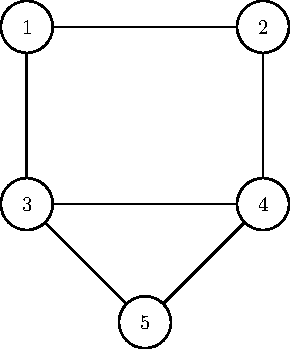
\includegraphics[scale=1]{graphs/max-cut-example.pdf}
	\centering
\end{figure}

We would have five variables: $x_1, \cdots, x_5$. The cost associated to edge $(1,2)$ is $x_1 + x_2 - 2 x_1 x_2$. By repeating this process for every edge in the graph we obtain the cost function:

$$ \text{Maximize  } f(x) = (x_1 + x_2 - 2 x_1 x_2) + (x_1 + x_3 - 2 x_1 x_3) + (x_2 + x_4 - 2 x_2 x_4) $$
$$ +(x_3 + x_4 - 2 x_3 x_4) + (x_3 + x_5 - 2 x_3 x_5) + (x_4 + x_5 - 2 x_4 x_5) $$

or equivalently:

$$ \text{Maximize  } f(x) = 2x_1 + 2x_2 + 3x_3 + 3x_4 + 2x_5$$ 
$$ - 2x_1x_2 - 2x_1x_3 - 2x_2x_4 - 2x_3x_4 - 2x_3x_5 - 2x_4x_5 $$

We can transform the problem using the following symmetric matrix:

$$
	Q = 
	\begin{pmatrix}
	2 & -1 & -1 & 0 & 0 \\
	-1 & 2 & 0 & -1 & 0 \\
	-1 & 0 & 3 & -1 & -1 \\
	0 & -1 & -1 & 3 & -1 \\
	0 & 0 & -1 & -1 & 2
	\end{pmatrix}
$$

Yielding the following compact form:

$$ \text{Maximize  } f_Q(x) = x^T Q x$$ 

The minimum value of $f_Q(x)$ is $x = (0, 1, 1, 0, 0)$. Thus, vertices $2$ and $3$ are in one set and vertices $1$, $4$ and $5$ are in the other one.


\subsection{General translation method}


The previous problem was naturally transform  into QUBO due to its particular constraints. However, can any quadratic optimization problem be encoded as a QUBO?

The answer is positive. Furthermore, any quadratic optimization problem with linear constraints may be transformed into a QUBO. Let us first study a simple case. Consider the following problem:

\begin{gather*}
	\text{Minimize } f(x_1, x_2) \\
	\text{subject to the constraint} \\
	x_1 + x_2 \leq 1
\end{gather*}

where $x_1, x_2 \in \B$. We may transform our linear constraint into a penalty $P(x_1x_2)$ for some positive scalar $P$. This term equals $0$ if and only if our constraint is satisfied by the variables. Thus, by adding the penalty to our cost function, for $P$ large enough, the problem

\begin{gather*}
	\text{Minimize } f(x_1, x_2) + Px_1x_2
\end{gather*}

will minimize $f(x_1, x_2)$ and, at the same time, satisfy the constraint. Namely, the constraint translates into adding a non-negativa value to the cost function. Some other useful translations can be found in table \ref{penalties-table}. In general, if the cost function is being minimized we may substitute constraints by non-negative terms that only equal zero if they are satisfied, multiplied by a large-enough positive value $P$. Thus, we may remove the associated constraints by simply adding these terms to the cost function. 

\begin{table}[h]
	\centering
	\begin{tabular}{cc}
		Classical Constraint 		& Equivalent Penalty   			\\ \hline
		$x + y \leq 1$       		& $P(xy)$              			\\
		$x + y \geq 1$       		& $P(1 - x - y + xy)$  			\\
		$x + y = 1$          		& $P(1 - x - y + 2xy)$ 			\\
		$x \leq y$       			& $P(x - xy)$      
		
		   			\\
		$x_1 + x_2 + x_3 \leq 1$	& $P(x_1x_2 + x_1x_3 + x_2x_3)$	\\
		$x = y$              		& $P(x + y - 2xy)$    
	\end{tabular}
	\caption{}
	\label{penalties-table}
\end{table}

Specifically, let us study the more general case:

$$ \text{Minimize } f(x) = x^T C x $$
$$ \text{subject to the constraints} $$
$$ Ax = b $$

where $x \in \B^n$, $k$ is the number of constraints, $b \in \R^k$, $C$ is a $n \times n$ matrix and $A$ is a $k \times n$ matrix. This accomodates to both linear and quadratic cost function since elements in the diagonal are $c_{ii} x_i^2 = c_{ii} x_i$. For a positive scalar $P$, the quadratic penalty $P (Ax - b)^T (Ax - b)$ is added to the cost function to obtain:

\begin{equation*}
	\begin{split}
		f'(x)	& = x^T C x + P (Ax - b)^T (Ax - b) \\
		& = x^T C x + P (x^TA^TAx - x^TA^Tb - b^TAx + b^Tb) \\
		& = x^T C x + x^T D x + c \\
		& = x^T Q x + c 
	\end{split}
\end{equation*}

where $D = P(A^TA)$, $c = P(- x^TA^Tb - b^TAx + b^Tb)$ and $Q = C + D$. Since the constant $c$ does not affect where the minimum is reached, $f$ and $f'$ share this minimum. Therefore, we may simply solve:

$$ \text{Minimize } f(x) = x^T Q x $$

which is a QUBO problem.

In this development we only considered equality constraints. There is also a general method to transform inequality constraints into equality ones by introducing \emph{slack variables} \cite{Hull2003}. In practice, the general case will not be necessary since the constraints are usually quite simple.

Finally, we may also consider satisfiability problems. That is, given a set of constrains for the variables, find a configuration of them such that all the constraints are satisfied. If the constraints are linear, these problems may be transformed into QUBO by setting the cost function as constant and following the same method. Suppose the constraints over $x$ can be written as $Ax = b$. The equivalent optimization problem is written as:

$$ \text{Minimize } f(x) = 0 $$
$$ \text{subject to the constraints} $$
$$ Ax = b $$

Any solution satisfaying the constraint will yield $0$ on the penalties, thus minimizing the transformed cost function $f'(x) = x^T Q x$. 

Let us explore some more complicated examples to expand this ideas.


\subsection{Graph Coloring}


Consider the following problem: Given a graph $G$ and $K$-colors, assign a single color to each vertex in $V$ such that no two adjacent vertices have the same color. Let $x_{ij}$ be a binary variable that is set to $1$ if and only if the $i$-th node is assigned the color $j$-th. We may develop the following two constraints. First, since all nodes must be colored exactly once:

$$ \sum_{j=1}^K x_{ij} = 1 \quad \forall i \in \{1, \cdots, n\} $$

where $n$ is the number of nodes. Moreover, the condition that two adjacent nodes cannot have the same color is translated into:

$$ x_{ic} + x_{jc} \leq 1 \quad \forall c \in \{1, \cdots, K\} $$

for every pair of adjancent nodes $(i,j)$ in $G$.

Thus, by finding a vector configuration for the variables $x_{ij}$ that satisfy this constraint, we find a solution of the graph coloring problem. This is what we introduced before as a satisfiability problem. Therefore, 
it may be written as:

$$ \text{Minimize } f(x) = 0 $$
$$ \text{subject to the constraints} $$
$$ \sum_{j=1}^K x_{ij} = 1 \quad \forall i \in \{1, \cdots, n\} \quad \text{and}$$
$$ x_{ic} + x_{jc} \leq 1 \quad \forall c \in \{1, \cdots, K\} \quad \text{for all adjacent nodes i and j}$$


\newparagraph{Numerical Example}


Given the following graph, find a coloring using three colors.

\begin{figure}[H]
	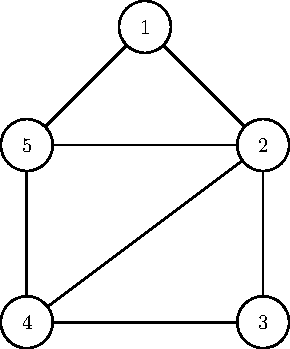
\includegraphics[scale=1]{graphs/graph-coloring-example.pdf}
	\centering
\end{figure}

For this particular graph there are $15$ variables $x_{ij}$ for all $i \in \{1, \cdots, 5\}$ and for all $j \in \{1, 2, 3\}$. The associated constraints are:

$$ x_{i1} + x_{i2} + x_{i3} = 1 \quad \forall i \in \{1, \cdots, 5\} $$
$$ x_{ic} + x_{jc} \leq 1 \quad \forall c \in \{1, 2, 3\} \quad \text{for all adjacent nodes i and j} $$

a total of $26$: $5$ for  assigning one and only one color to each node, and $3$ additional ones per edge in the graph ($7$) for no adjacent equally colored nodes. First, let us rename our variables from $1$ to $15$ as follows:

$$ (x_{11}, x_{12}, x_{13}, x_{21}, x_{22}, x_{23}, x_{31}, \dots, x_{52}, x_{53}) =
	(x_1, x_2, x_3, x_4, x_5, x_6, x_7, \dots, x_{15}, x_{16}) $$

The first set of constraints may be substitued by $P(x_{i1} + x_{i2} + x_{i3} - 1)^2$, which only equals $0$ if the constraint is satisfied. For instance, for the first node $P(x_1 + x_2 + x_3 - 1)^2$ is tranformed to $P(- x_1 - x_2 - x_3 + 2 x_1 x_2 + 2 x_1 x_3 + 2 x_2 x_3) + P$. By chosing a value for $P=4$ and dropping the constant we can  insert these penalties into an under developed $Q$ matrix:

$$
Q = 
\left(
\begin{array}{*{15}c}
	-4 & 4 & 4 & 0 & 0 & 0 & 0 & 0 & 0 & 0 & 0 & 0 & 0 & 0 & 0 \\
	4 & -4 & 4 & 0 & 0 & 0 & 0 & 0 & 0 & 0 & 0 & 0 & 0 & 0 & 0 \\
	4 & 4 & -4 & 0 & 0 & 0 & 0 & 0 & 0 & 0 & 0 & 0 & 0 & 0 & 0 \\
	0 & 0 & 0 & -4 & 4 & 4 & 0 & 0 & 0 & 0 & 0 & 0 & 0 & 0 & 0 \\
	0 & 0 & 0 & 4 & -4 & 4 & 0 & 0 & 0 & 0 & 0 & 0 & 0 & 0 & 0 \\
	0 & 0 & 0 & 4 & 4 & -4 & 0 & 0 & 0 & 0 & 0 & 0 & 0 & 0 & 0 \\
	0 & 0 & 0 & 0 & 0 & 0 & -4 & 4 & 4 & 0 & 0 & 0 & 0 & 0 & 0 \\
	0 & 0 & 0 & 0 & 0 & 0 & 4 & -4 & 4 & 0 & 0 & 0 & 0 & 0 & 0 \\
	0 & 0 & 0 & 0 & 0 & 0 & 4 & 4 & -4 & 0 & 0 & 0 & 0 & 0 & 0 \\
	0 & 0 & 0 & 0 & 0 & 0 & 0 & 0 & 0 & -4 & 4 & 4 & 0 & 0 & 0 \\
	0 & 0 & 0 & 0 & 0 & 0 & 0 & 0 & 0 & 4 & -4 & 4 & 0 & 0 & 0 \\
	0 & 0 & 0 & 0 & 0 & 0 & 0 & 0 & 0 & 4 & 4 & -4 & 0 & 0 & 0 \\
	0 & 0 & 0 & 0 & 0 & 0 & 0 & 0 & 0 & 0 & 0 & 0 & -4 & 4 & 4 \\
	0 & 0 & 0 & 0 & 0 & 0 & 0 & 0 & 0 & 0 & 0 & 0 & 4 & -4 & 4 \\
	0 & 0 & 0 & 0 & 0 & 0 & 0 & 0 & 0 & 0 & 0 & 0 & 4 & 4 & -4 
\end{array}
\right)
$$

Secondly, in order to transform $x + y \leq 1$ we can refer to table \ref{penalties-table} and use $P(xy)$. We add these penalties to the previous matrix in the proper places:

$$
Q = 
\left(
\begin{array}{*{15}c}
-4 & 4 & 4 & 2 & 0 & 0 & 0 &
% TODO: rephrasear la cita en el contexto anterior



 0 & 0 & 0 & 0 & 0 & 2 & 0 & 0 \\
4 & -4 & 4 & 0 & 2 & 0 & 0 & 0 & 0 & 0 & 0 & 0 & 0 & 2 & 0 \\
4 & 4 & -4 & 0 & 0 & 2 & 0 & 0 & 0 & 0 & 0 & 0 & 0 & 0 & 2 \\
2 & 0 & 0 & -4 & 4 & 4 & 2 & 0 & 0 & 2 & 0 & 0 & 2 & 0 & 0 \\
0 & 2 & 0 & 4 & -4 & 4 & 0 & 2 & 0 & 0 & 2 & 0 & 0 & 2 & 0 \\
0 & 0 & 2 & 4 & 4 & -4 & 0 & 0 & 2 & 0 & 0 & 2 & 0 & 0 & 2 \\
0 & 0 & 0 & 2 & 0 & 0 & -4 & 4 & 4 & 2 & 0 & 0 & 0 & 0 & 0 \\
0 & 0 & 0 & 0 & 2 & 0 & 4 & -4 & 4 & 0 & 2 & 0 & 0 & 0 & 0 \\
0 & 0 & 0 & 0 & 0 & 2 & 4 & 4 & -4 & 0 & 0 & 2 & 0 & 0 & 0 \\
0 & 0 & 0 & 2 & 0 & 0 & 2 & 0 & 0 & -4 & 4 & 4 & 2 & 0 & 0 \\
0 & 0 & 0 & 0 & 2 & 0 & 0 & 2 & 0 & 4 & -4 & 4 & 0 & 2 & 0 \\
0 & 0 & 0 & 0 & 0 & 2 & 0 & 0 & 2 & 4 & 4 & -4 & 0 & 0 & 2 \\
2 & 0 & 0 & 2 & 0 & 0 & 0 & 0 & 0 & 2 & 0 & 0 & -4 & 4 & 4 \\
0 & 2 & 0 & 0 & 2 & 0 & 0 & 0 & 0 & 0 & 2 & 0 & 4 & -4 & 4 \\
0 & 0 & 2 & 0 & 0 & 2 & 0 & 0 & 0 & 0 & 0 & 2 & 4 & 4 & -4 
\end{array}
\right)
$$

Since the matrix above incorporate all the constraints, finding a graph coloring is equivalent to finding a minimum of:

$$ \text{Minimize } f(x) = x^T Q x $$

Solving this model yields $x_2 = x_4 = x_9 = x_{11} = x_{15} = 1$, and $0$ for the rest of the variables. Meaning, nodes $1$ and $4$ are assigned color number $2$, node $2$ is assigned color number $1$, and nodes $3$ and $5$ are assigned color number $3$.

As a final remark, this method of graph coloring has proven to be computationally useful for graphs with up to $450$ nodes and $9757$ edges \cite{Kochenberger2005}.


\subsection{The Travelling Salesman problem}


In order to formulate our next problem, a couple of extra definitions are needed. Given a graph, a \emph{Hamiltonian path} is a path -a sequence of conected nodes- such that it only passes through each node exactly once. A \emph{cycle}, also called \emph{tour}, is a path that starts and ends in the same node. A \emph{Hamiltonian cycle} is a cycle that passes through each node a single time, except for the first/last node which appears twice in the cycle. Additionally, a weighted graph $G =(V, E, W)$ is a graph with a series of weigths $w_e \in \R$ associated to each edge $e \in E$.

The Travelling Salesman problem is the following: Given a directed weighted graph, find a Hamiltonian cycle with minimum total weight. The problem is sometimes stated with a Hamiltonian path instead of Hamiltonian cyle, but as it will be seen in section [TODOref], for our pourposes the cycle-statement will be of better use.

We may supposse without lossing generality that the graph is complete. That is, there is always an edge from every two nodes in every direction. If the given graph is not complete, we may add the remaining edges with a high enough weigth so that they are never used.

Since solutions to this problem are a series of $n \equiv |V|$ nodes -the number of nodes in the graph-, we will encode $n$-nodes cycles as $(v_{k_0}, \ldots, v_{k_{n-1}})$, where nodes $e_{k_0}$ and $e_{k_{n-1}}$ are also conected. Thus, our problem may originally may stated as:

$$ \text{Minimize } \sum_{i=0}^{n-1} w_{k_i, k_{i+1}} $$
$$ \text{subject to the constraint that } (v_{k_0}, \cdots, v_{k_{n-1}}) \text{ is a Hamiltonian cycle}$$

where the $k_n \equiv k_0$. The binary variables $x_{i,p}$ will be used, where $i,p \in \{0, \ldots, n-1\}$. $x_{i,p}$ will equal $1$ if and only if node $i$ is in position $p$ in our cycle. Thus, we will have $n^2$ variables under the following constraints:

\begin{enumerate}
	\item Every node must be assigned. Thus, node assigment will be rewarded with a non-positive weight (favorable bias) called \textbf{self-bias} with an associated non-positive penalty:
	
	$$ a x_{i,p} \quad \forall i,p \in \{0, \ldots, n-1\} $$
	
	where $a \leq 0$. In practice, this will not be necessary for every problem. We may remove the self-bias by setting $a=0$. Adding these penalties for every node and position yields:
	
	\begin{equation}
		\label{eqn:salesman-constrain1}
		a \sum_{i=0}^{n-1} \sum_{p=0}^{n-1} x_{i,p}
	\end{equation}
	
	\item Every node must be assigned to only one position. This constraint will be called \textbf{repetition}:
	
	$$ \sum_{p=0}^{n-1} x_{i,p} = 1 \quad \forall p \in \{0, \ldots, n-1\} $$
	
	Resulting in the following penalty:
	
	$$ b \Big( \sum_{p=0}^{n-1} x_{i,p} - 1 \Big)^2 \quad \forall p \in \{0, \ldots, n-1\} $$

	where $b$ is a positive parameter. Adding these $n$ penalties we obtain:
	
	\begin{equation}
		\label{eqn:salesman-constrain2}
		b \sum_{i=0}^{n-1} \Big( \sum_{p=0}^{n-1} x_{i,p} - 1 \Big)^2
	\end{equation}
		
	\item Every position must be assigned only one node. This constraint will be called \textbf{colocation}:
	
	$$ \sum_{i=0}^{n-1} x_{i,p} = 1 \quad \forall i \in \{0, \ldots, n-1\} $$
	
	Resulting in the following penalty:
	
	\begin{equation}
		\label{eqn:salesman-constrain3}
		c \sum_{p=0}^{n-1} \Big( \sum_{i=0}^{n-1} x_{i,p} - 1 \Big)^2
	\end{equation}
	
	where $c$ is a positive parameter.	
\end{enumerate}

Finally, we may re-write the cost function in terms of the binary variables. Weight $w_{ij}$ must be added in the cost function if and only if nodes $i$ and $j$ follow each other in the path. That is, if and only if $x_{i,p}x_{j,p+1} = 1$ for any position $p$. In fact, it may be needed to add it multiple times if the previous equality holds for multiple positions. Thus, the penalty associated to weight $w_{i,j}$ is:

$$ w_{i,j} \sum_{p=0}^{n-1} x_{i,p}x_{j,p+1} $$

Adding up the penalties associated to every weigth yields the cost function:

$$ \text{Minimize } \sum_{i=0}^{n-1} \sum_{j=0}^{n-1} w_{i,j}\sum_{p=0}^{n-1} x_{i,p}x_{j,p+1} $$

The final QUBO model is obtained by adding the penalties \ref{eqn:salesman-constrain1}, \ref{eqn:salesman-constrain2} and \ref{eqn:salesman-constrain3} to the cost function:

% Using an extra column for left aligment.
\begin{equation}
	\begin{alignedat}{3}
		& \text{Minimize }	&& \sum_{i=0}^{n-1} \sum_{j=0}^{n-1} w_{i,j}\sum_{p=0}^{n-1} x_{i,p}x_{j,p+1} & \\
		& && + a \sum_{i=0}^{n-1} \sum_{p=0}^{n-1} x_{i,p} & \qquad \text{(self-bias)} \\
		& && + b \sum_{i=0}^{n-1} \Big( \sum_{p=0}^{n-1} x_{i,p} - 1 \Big)^2 & \qquad \text{(repetition)} \\
		& && + c \sum_{p=0}^{n-1} \Big( \sum_{i=0}^{n-1} x_{i,p} - 1 \Big)^2 & \qquad \text{(colocation)}
	\end{alignedat}
	\label{eqn:salesman-cost-funct}
\end{equation}


Since this is a quadratic unconstraint function, this is already a QUBO. The conversion to matrix is straight-forward. Let us see this in an example.


\newparagraph{Numerical Example}


Given the following graph:

\begin{figure}[H]
	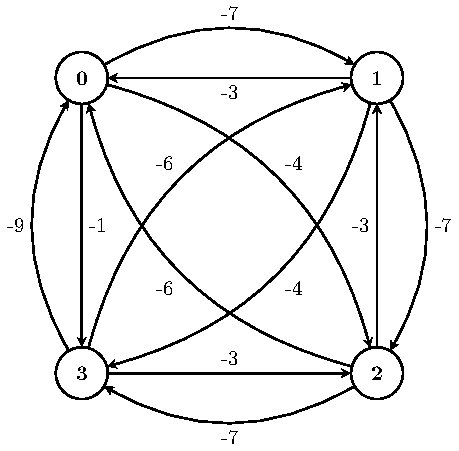
\includegraphics[scale=1.1]{graphs/salesman-example.pdf}
	\centering
\end{figure}

Find a Hamiltonian cycle with minimum cost. 

First of all, let us take a deeper look into our possible solutions. There are $(n-1)!$ cycles in a graph with $n$ nodes. For our $4$-nodes graph there are $3! = 6$ type of cycles:

\begin{itemize}
	\item Type A: $0 \rightarrow 1 \rightarrow 2 \rightarrow 3 \rightarrow 0$
	\item Type B: $0 \rightarrow 3 \rightarrow 2 \rightarrow 1 \rightarrow 0$
	\item Type C: $0 \rightarrow 2 \rightarrow 1 \rightarrow 3 \rightarrow 0$
	\item Type D: $0 \rightarrow 3 \rightarrow 1 \rightarrow 2 \rightarrow 0$
	\item Type E: $0 \rightarrow 1 \rightarrow 3 \rightarrow 2 \rightarrow 0$
	\item Type F: $0 \rightarrow 2 \rightarrow 3 \rightarrow 1 \rightarrow 0$
\end{itemize}

We may see this graphically in table \ref{tbl:salesman-cycles}.

\begin{table}[H]
	\centering
	\begin{tabular}{ccc}		
		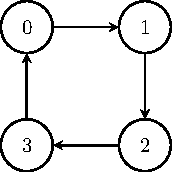
\includegraphics[scale=1]{graphs/salesman-cycleA.pdf} &
		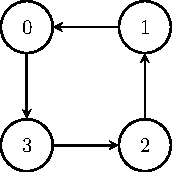
\includegraphics[scale=1]{graphs/salesman-cycleB.pdf} &
		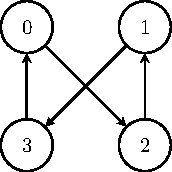
\includegraphics[scale=1]{graphs/salesman-cycleC.pdf} \\
		
		Type A & Type B & Type C \\
		
		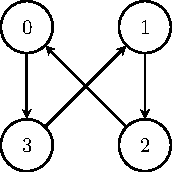
\includegraphics[scale=1]{graphs/salesman-cycleD.pdf} &
		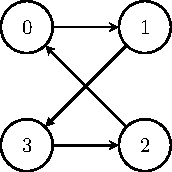
\includegraphics[scale=1]{graphs/salesman-cycleE.pdf} &
		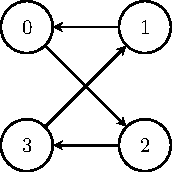
\includegraphics[scale=1]{graphs/salesman-cycleF.pdf} \\
		
		Type D & Type E & Type F \\
	\end{tabular}
	\caption{Type of cycles in a $4$-nodes graph}
	\label{tbl:salesman-cycles}
\end{table}

These six are the only possible cycles through our graph and of them will be the one with minimum cost. Since our binary encoding additionally depends on the node position, there are $4$ solutions of our encoding that represent the same cycle. For example, ($0 \rightarrow 1 \rightarrow 2 \rightarrow 3 \rightarrow 0$) and ($1 \rightarrow 2 \rightarrow 3 \rightarrow 0 \rightarrow 1$) both represent cycle type A. In this case, type A will be the tour with minimum cost.

A graphical representation of the different penalties interactions is shown in figure \ref{fig:salesman-penalties}, based on the constraints defined above.

\begin{table}[]
	\centering
	\makebox[\textwidth][c]{
		\begin{tabular}{ccc}		
			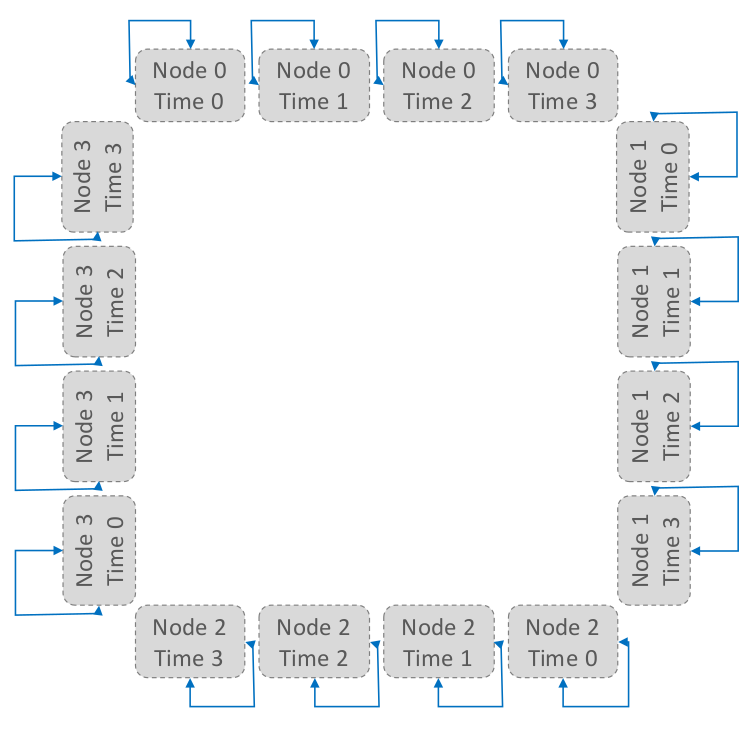
\includegraphics[scale=0.2]{salesman-penalties1.png} &
			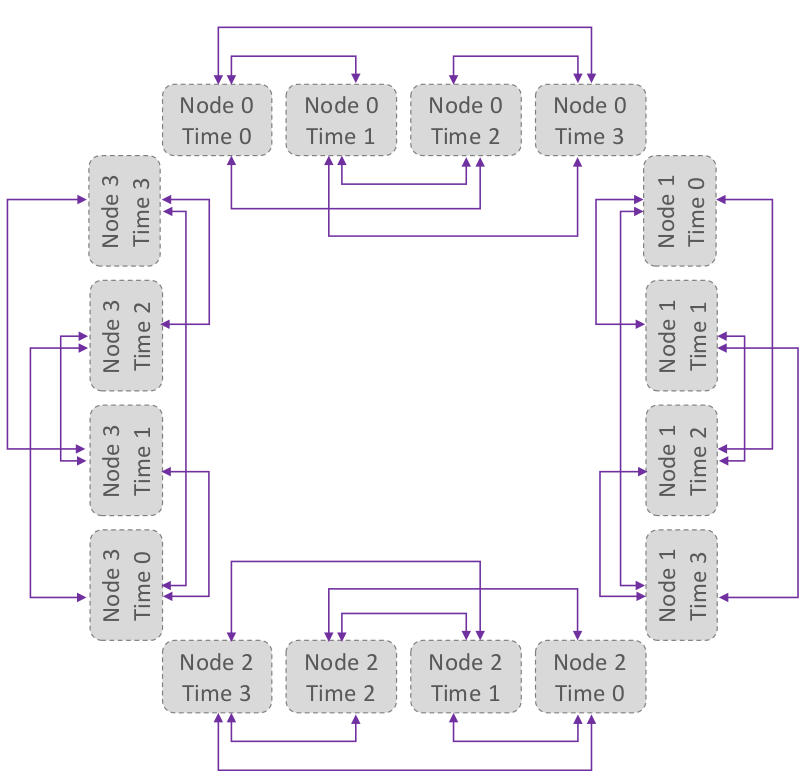
\includegraphics[scale=0.2]{salesman-penalties2.png} &
			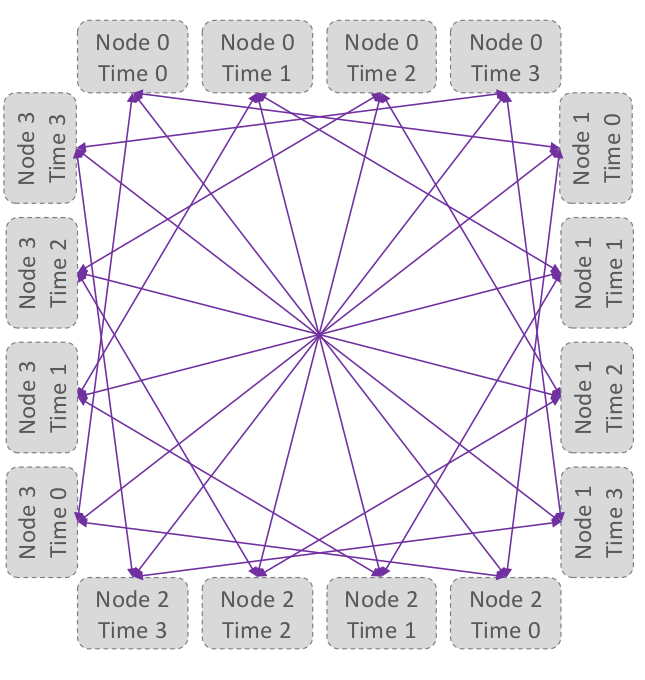
\includegraphics[scale=0.2]{salesman-penalties3.png} \\
			
			1: Self-bias & 2: Repetition & 3: Colocation \\
			
			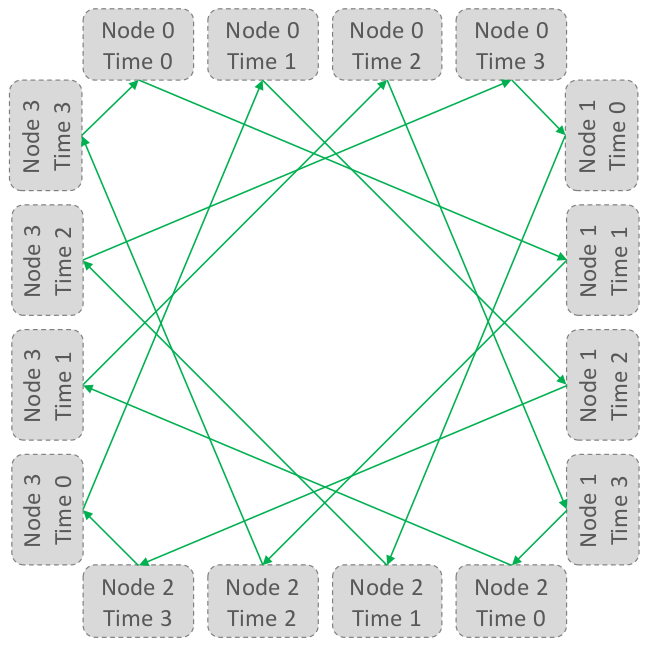
\includegraphics[scale=0.2]{salesman-penalties4.png} &
			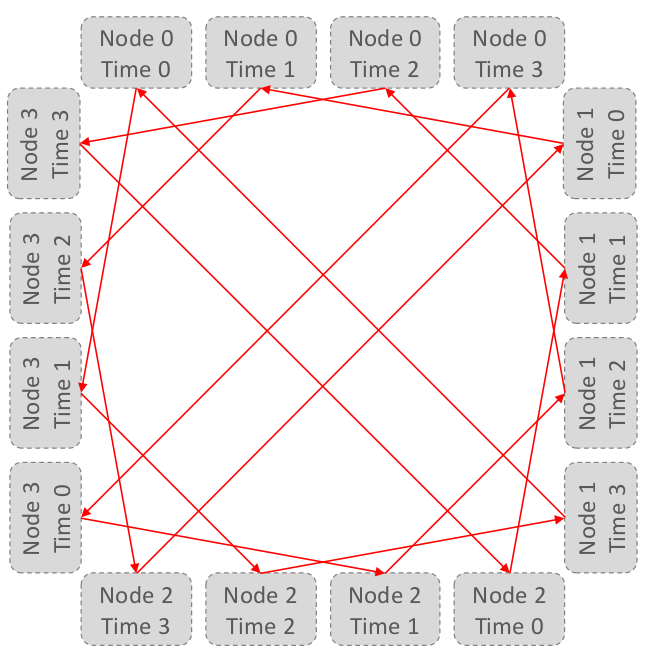
\includegraphics[scale=0.2]{salesman-penalties5.png} &
			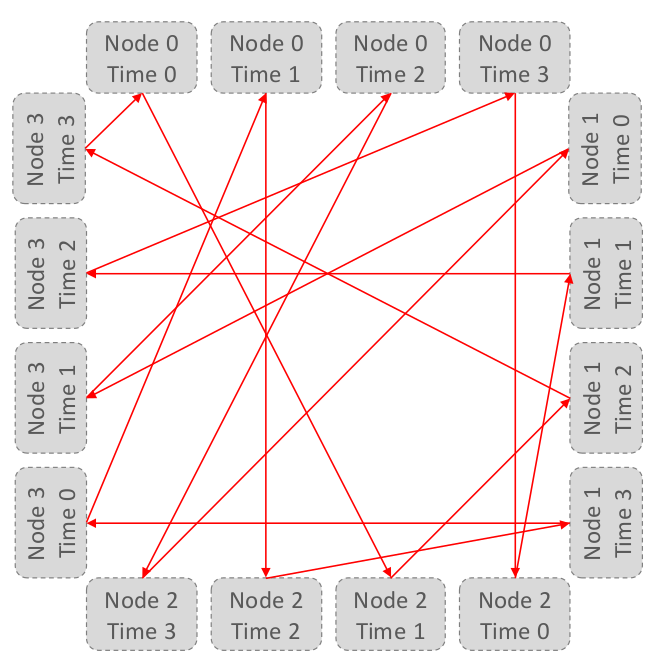
\includegraphics[scale=0.2]{salesman-penalties6.png} \\
			
			4: Type A tours & 5: Type B tours & 6: Type C tours \\
			
			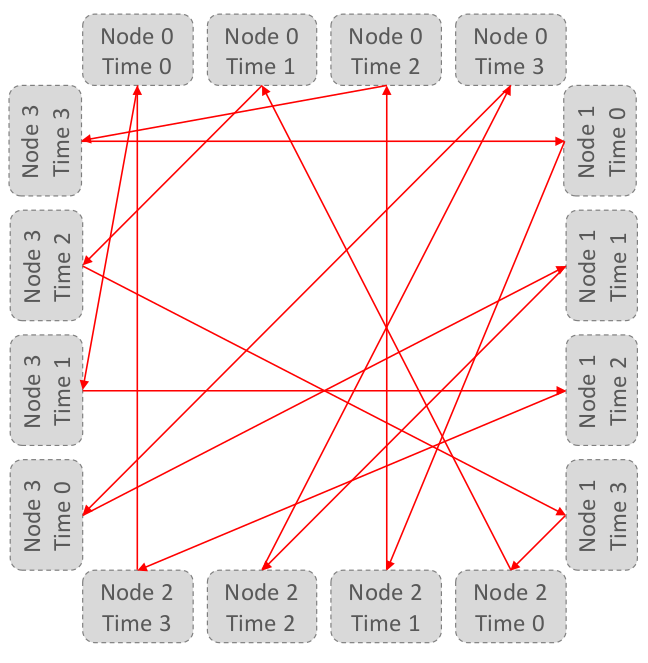
\includegraphics[scale=0.2]{salesman-penalties7.png} &
			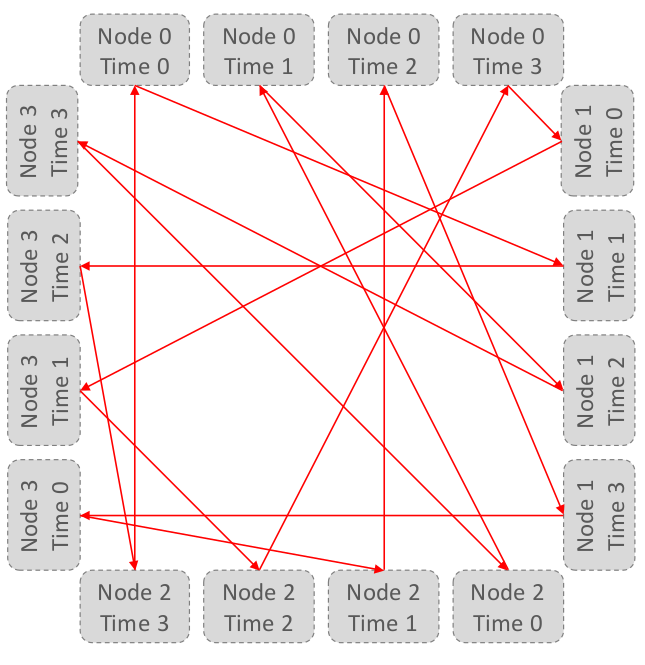
\includegraphics[scale=0.2]{salesman-penalties8.png} &
			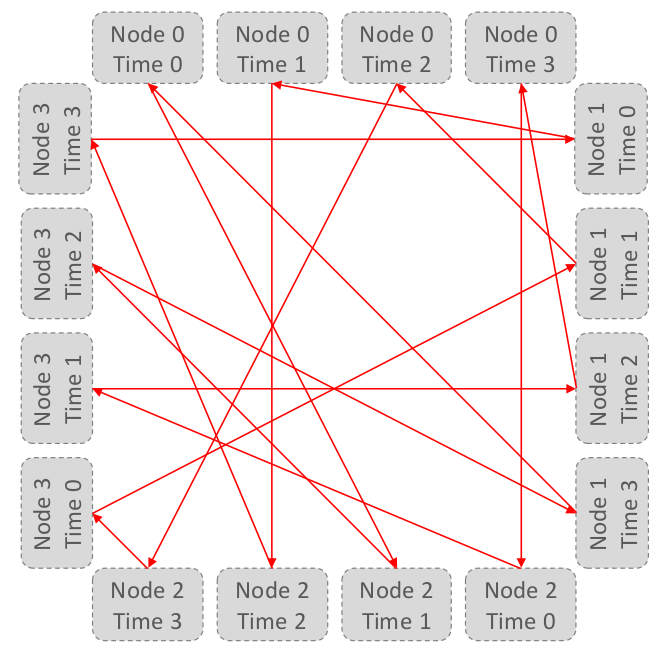
\includegraphics[scale=0.2]{salesman-penalties9.png} \\
			
			7: Type D tours & 8: Type E tours & 9: Type F tours \\
		\end{tabular}
	}
	\caption{Graphical representation of penalties between interactions \cite{Sarkar2020}}
	\label{fig:salesman-penalties}
\end{table}

We start the problem refactoring by renaming the variables:

$$ (x_{0,0}, x_{0,1}, x_{0,2}, x_{0,3}, x_{1,0}, x_{1,1}, x_{1,2}, \dots, x_{3,2}, x_{3,3}) =
(x_1, x_2, x_3, x_4, x_5, x_6, x_7, \dots, x_{15}, x_{16}) $$

Each of the terms in the cost function \ref{eqn:salesman-cost-funct} may be transformed into a matrix. The term associated to the weights is additionally splitted using the different types of cycles in which they appear. We thus obtain nine adjacency matrices, found on figure \ref{fig:salesman-adj-matrices}.

\begin{figure}[H]
	\makebox[\textwidth][c]{
		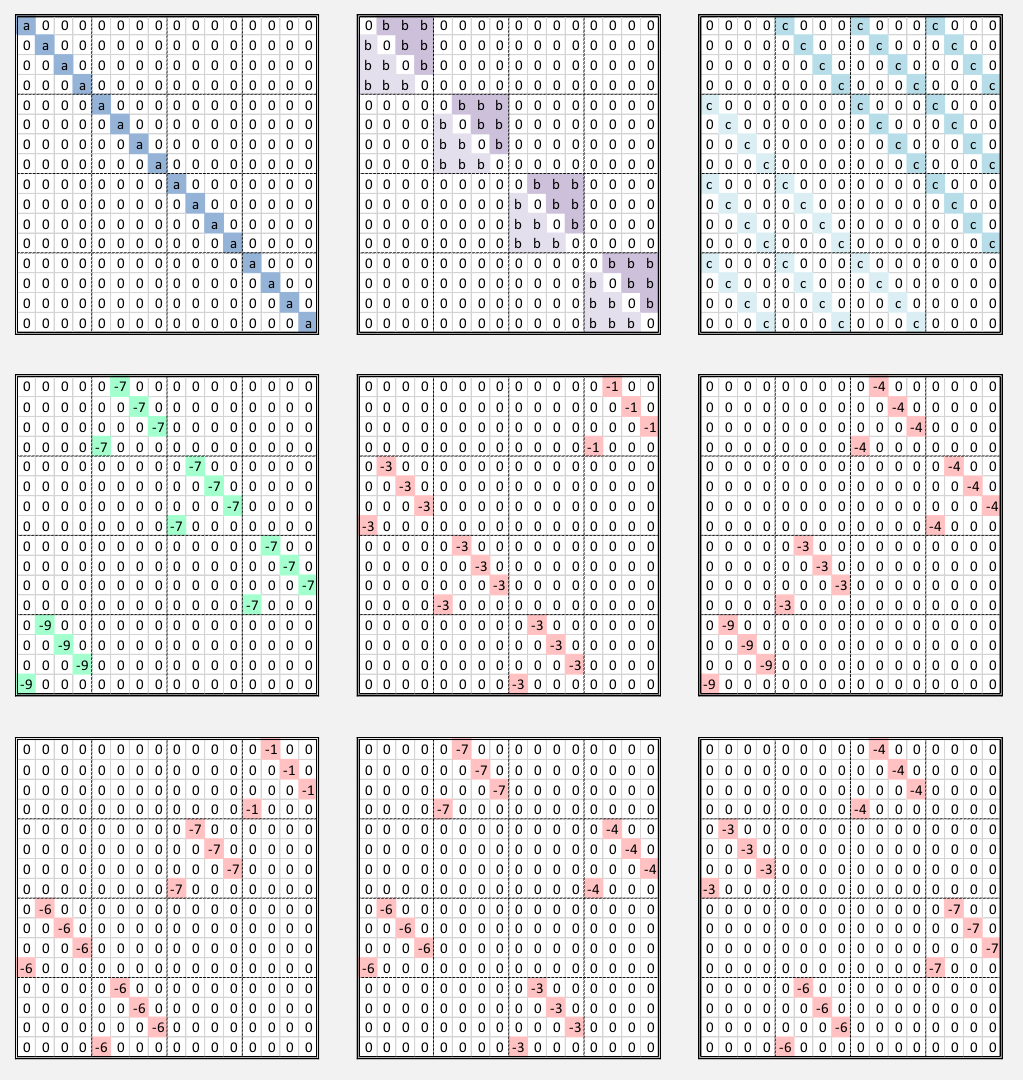
\includegraphics[scale=0.5]{salesman-adj-matrices.png}
	}
	\centering
	\label{fig:salesman-adj-matrices}
	\caption{Caption}
\end{figure}

Note that the matrices associated with the constraints are all symmetric since they only depend on the graph topology and not on the weights. On the other hand, since the cost of going back and forth between a pair of nodes is never the same, the matrices associated with the cycles are never symmetric.

% TODO: Finish the example


\subsection{3-SAT}


% TODO finish section
% TODO fix sources of each example


\section{D-Wave Systems}


\textbf{D-Wave Systems Inc.} is a Canadian company dedicated to quantum computing. In 2011, they announced the first commercial quantum computer system, D-Wave One. During the following two decades, the D-Wave team have developed a series of computing computers dedicated to quantum annealing. The last one being the Advantage System (figure \ref{fig 2.2}).

\begin{figure}[h]
	\includegraphics[scale=.1]{advantage_system.png}
	\centering
	\caption{Advantage$^{TM}$ system}.
	\label{fig 2.2}
\end{figure}

The quantum processing unit (QPU) of this system consist of $5640$ qubits and $40,484$ \emph{couplers} (links between qubits that allow entanglement between a pair of qubits). The number of couplers is especially relevant. It tells us that not every qubit can be entangled with every other qubit. We will come back to this in section [TODOref]. Since the QPU must be isolated to operate, it is encapsulated in a system at temperatures below 15 mK. In addition, radio frequency (RF)-shielded enclousre and magnetic shieldings are used to protect it from electromagnetic interferience \cite{DWaveDoc}.

\begin{figure}[h]
	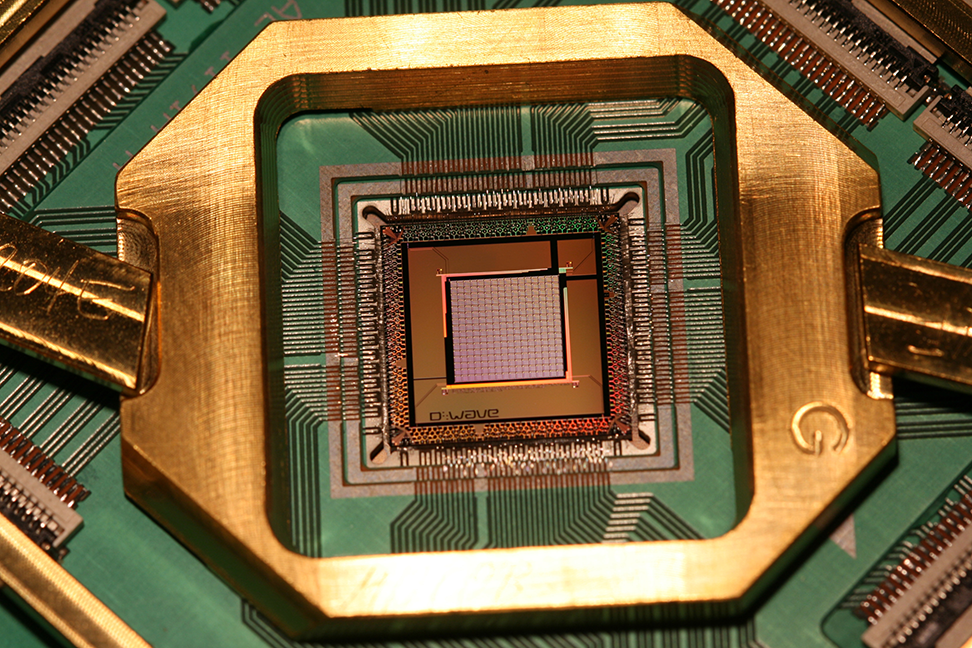
\includegraphics[scale=.2]{qpu.png}
	\centering
	\caption{D-Wave QPU}.
	\label{fig 2.3}
\end{figure}

D-Wave provides an easy-to-use software enviroment to solve problems using quantum annealing. We will explain in depth in section [TODOref].


\subsection{Quantum Annealing in D-Wave}
\label{quantum-annealing-dwave}


For this section we refer to the D-Wave documentation, which explains how quantum annealing is implemented and may be exploited in the D-Wave systems \cite{DWaveDoc-QuantumAnnealing}.


% TODO: rephrasear la cita en el contexto anterior
% TODO: change fig labels in this section











https://journals.aps.org/prl/pdf/10.1103/PhysRevLett.117.180402




